% LipScribe final technical report (W4-11 skeleton, F-11).
% Template: IEEE Access, as in the project proposal. Copy ieeeaccess.cls, the logo files
% (logo.png, notaglinelogo.png, bullet.png) and the spotcolor/T1-font files from the proposal's
% Overleaf project into this folder before compiling.
% Build: latexmk -pdf main.tex
% Each section file names its author; the editor is Lisa Lusinga Namugenyi.
\documentclass{ieeeaccess}
\usepackage{cite}
\usepackage{amsmath,amssymb,amsfonts}
\usepackage{graphicx}
\usepackage{textcomp}
\usepackage{booktabs}
\usepackage{url}
\def\BibTeX{{\rm B\kern-.05em{\sc i\kern-.025em b}\kern-.08em
    T\kern-.1667em\lower.7ex\hbox{E}\kern-.125emX}}

\begin{document}
\history{Date of publication xxxx 00, 0000, date of current version xxxx 00, 0000.}
\doi{10.1109/ACCESS.2026.DOI}

\title{LipScribe: Lip-Assisted Speech Recognition for Robust Live Captioning}

\author{\uppercase{Cole Rodney Migisha}\authorrefmark{1},
\uppercase{Charis Opol}\authorrefmark{1},
\uppercase{Ainomugisha Faith}\authorrefmark{1},
\uppercase{Lisa Lusinga Namugenyi}\authorrefmark{1},
\uppercase{Ansasire Nehum Naamaye}\authorrefmark{1},
and \uppercase{Wakisa Isabelle}\authorrefmark{1}}

\address[1]{Department of Computer Science, Uganda Christian University, Mukono, Uganda
(e-mail: \{b29657, b29654, b27518, b30300, b29785, b30311\}@students.ucu.ac.ug)}

\tfootnote{This work is submitted as the final technical report of the LipScribe project in the
Computer Vision and Deep Learning course, Group~4.}

\markboth
{Migisha \headeretal: LipScribe: Lip-Assisted Speech Recognition for Robust Live Captioning}
{Migisha \headeretal: LipScribe: Lip-Assisted Speech Recognition for Robust Live Captioning}

\corresp{Corresponding author: Cole Rodney Migisha (e-mail: b29657@students.ucu.ac.ug).}

% Author: Lisa Lusinga Namugenyi (editor). Write last, after the results are final (F-11).
\begin{abstract}
% TODO (F-11): 150-250 words. Problem; approach (lip-assisted audio-visual speech recognition with
% cross-modal attention, gated fusion and modality dropout); GRID results of model P4 at five
% noise levels; real-world results of ws_v5 on films and TED; the live demo; one limitation.
\end{abstract}

\begin{keywords}
Audio-visual speech recognition, lip reading, multimodal fusion, cross-modal attention,
connectionist temporal classification, live captioning, noise robustness.
\end{keywords}


\titlepgskip=-21pt

\maketitle

% Author: Charis Opol. Reuse and update the proposal's introduction (F-11).
\section{Introduction}
\label{sec:introduction}
% TODO (F-11): motivation (captioning in noisy rooms, accessibility); why the lips help when the
% audio fails; the research questions: (1) does lip-assisted fusion help on GRID across noise
% levels, (2) does it carry over to real speech; contributions; outline of the report.

% Author: Charis Opol. Reuse and update the proposal's related work (F-11).
\section{Related Work}
\label{sec:related}
% TODO (F-11): lip reading (LipNet, Stafylakis and Tzimiropoulos~\cite{stafylakis2017},
% Martinez et al.~\cite{martinez2020}); audio-visual speech recognition (Auto-AVSR~\cite{ma2023});
% self-supervised audio (WavLM~\cite{chen2022wavlm}); CTC~\cite{graves2006}; datasets
% (GRID~\cite{cooke2006}, LRS3~\cite{afouras2018}).

% Author: Ainomugisha Faith (first draft written 16 Nov from the repository; check and extend).
\section{Data and Noise}
\label{sec:data}

\subsection{GRID corpus}
LipScribe is trained and tested on the GRID audio-visual corpus~\cite{cooke2006}. Every GRID
sentence follows a six-slot command grammar (command, colour, preposition, letter, digit,
adverb) drawn from 51 words, and lasts 3~s: 75 video frames at 25~frames/s with 16~kHz audio.
The team verified every utterance before use (\texttt{scripts/verify\_dataset.py}): video,
audio and alignment files present; $75 \pm 2$ decodable frames; audio duration within 40~ms of
the video; a six-word transcript from the GRID word list; audio neither silent nor clipped
throughout; and a Face Mesh success rate of at least 90~\% of frames.

The split is speaker-independent (\texttt{data/splits.csv}), so no test speaker is ever seen in
training: 26 speakers for training (25,891 usable utterances), 3 for validation (3,000) and 4
for testing (3,999), 32,890 in total. Speaker s21 is excluded because its video is missing.
The split was fixed in Week~1 and never regenerated.

\subsection{Noise}
Background noise comes from the MUSAN corpus~\cite{snyder2015}. Its 930 noise files are split
by file into separate pools for training (651), validation (139) and testing (140), so no noise
recording appears in more than one pool. During training each utterance is mixed with a random
training-pool segment at a signal-to-noise ratio (SNR) drawn uniformly from clean, 10, 5, 0 and
$-5$~dB. Validation and test use fixed noisy copies of every utterance at the same five levels,
made once with deterministic seeds (\texttt{scripts/make\_noisy\_test.py}), so every model is
scored on identical audio. After mixing, each waveform is scaled to $-25$~dBFS RMS with the
gain capped at 20~dB, so near-silent clips are not amplified into pure noise.

\subsection{Real-world data}
% TODO (Faith, F-11): two short paragraphs on the out-of-domain data used for the real-world
% model: subtitled films and series mined into GRID-format clips (scripts/mine_flix.py; one
% visible, frontal speaker per clip), films without subtitles and TED talks labelled by Whisper
% word timestamps, the download-mine-delete harvester (only mouth crops are kept), and the
% film/TED train, validation and test splits (test titles and talks never used in training).
% Numbers: reports/flix_v5/decision_log.md (manifest counts) and the Week 4 report.

% Author: Cole Rodney Migisha (first draft written 16 Nov from the repository; check and extend).
\section{Visual and Audio Pipelines}
\label{sec:pipelines}

\subsection{Mouth crops}
The visual input is a sequence of grey $96 \times 96$ mouth crops at 25~frames/s
(\texttt{lipscribe/preprocessing/crop.py}). MediaPipe Face Mesh finds the lip landmarks in every
frame; a square box around them, enlarged by a 25~\% margin, is smoothed over time with a
centred moving average, and frames where the face is lost take the box of their neighbours.
The crop is padded by repeating edge pixels when the box leaves the frame, and a per-frame
validity mask records where Face Mesh succeeded. The model therefore always receives 75 frames
per GRID clip, and knows which of them show a real face.

During training the crops are augmented with a random shift of up to 4 pixels, a horizontal
flip with probability 0.5, a scale change of up to 10~\%, a random erased patch (probability
0.5, up to 15~\% of the area) and two time masks of up to 6 frames each. Evaluation and the
application use the crops unchanged.

\subsection{Audio features}
Audio is resampled to 16~kHz mono and converted on the GPU to 80-band log-Mel features with a
25~ms window, a 10~ms hop and a 512-point FFT, then standardised with the mean and standard
deviation of the training set (\texttt{lipscribe/preprocessing/features.py}). Experiment X5
compared these features with 39 MFCCs and with log-Mel plus MFCC on the audio-only baseline;
log-Mel plus MFCC lowered the mean validation WER from 7.72~\% to 6.90~\%
(\texttt{reports/w3\_08\_audio\_features\_decision.md}).
% TODO (Cole): say whether P4 keeps log-Mel 80 (it does: configs/p_init_b1_b2_v2.yaml) and why.

\subsection{Encoders}
The audio encoder applies two strided 1-D convolutions ($80 \rightarrow 256 \rightarrow 256$,
kernel~3, stride~2), which reduce the 100~frames/s features to the video rate of 25~frames/s,
followed by a two-layer bidirectional LSTM with 256 units per direction. Both visual encoders
map $[B, 1, T, 96, 96]$ crops to $[B, T, 512]$. V1 stacks three 3-D convolution blocks (32, 64
and 96 channels) before a linear layer and a two-layer BiLSTM. V2 follows the lip-reading
front end of Stafylakis and Tzimiropoulos~\cite{stafylakis2017}: one $5 \times 7 \times 7$ 3-D
convolution, a ResNet-18 trunk applied to each frame, and the same BiLSTM. V2 learned faster
and generalised better, so model P4 uses it.

\subsection{Real-world pipeline}
% TODO (Cole, F-11): the v4-v6 pipeline: Auto-AVSR-style mouth crops, WavLM Base+ audio
% encoder~\cite{chen2022wavlm}, Auto-AVSR visual encoder~\cite{ma2023}, word-piece CTC; the
% audio-only twin and the reliability-gated warm start (ws_v5); the v5 re-cut with 0.32 s
% padding and Whisper word-timestamp labels. Sources: reports/flix_v5/decision_log.md.

% Author: Charis Opol (first draft written 16 Nov from the repository; check and extend).
\section{Model and Training}
\label{sec:model}

\subsection{Baselines}
Three baselines frame the proposed model. B1 hears only the audio, B2 sees only the lips, and
B3 joins the two encoders by concatenating their features frame by frame. All models end in
the same connectionist temporal classification (CTC) head~\cite{graves2006} over 28 symbols:
the 26 letters, the space and the CTC blank.

\subsection{Proposed model P}
Model P projects each stream from 512 to 256 dimensions with layer normalisation, then lets
each stream attend to the other with bidirectional cross-modal attention (four heads,
$d = 256$, attention dropout 0.1, residual connections and layer normalisation). A per-frame
gate then weighs the two attended streams:
\begin{equation}
g_t = \sigma\big(W [\tilde{a}_t; \tilde{v}_t] + b\big), \qquad
f_t = g_t\, \tilde{a}_t + (1 - g_t)\, \tilde{v}_t ,
\end{equation}
so $g_t$ close to 1 means the model trusts the sound and close to 0 that it trusts the lips.
A learned 256-dimensional vector $e_{\text{miss}}$ replaces a stream that is missing. During
training, modality dropout replaces the audio with $e_{\text{miss}}$ for 25~\% of utterances
and the video for 15~\%, never both at once, so the model learns to work with either stream
alone. At inference, a clip whose face is missing in more than half of its frames uses
$e_{\text{miss}}$ for the video.

\subsection{Training}
All models train with AdamW (learning rate $3 \times 10^{-4}$, weight decay $10^{-2}$), batch
size 16, one warm-up epoch followed by a cosine schedule, gradient clipping at 5 and mixed
precision, for up to 40 epochs. Early stopping watches the mean validation WER over the five
SNR levels, with a patience of 12 epochs, and the checkpoint with the lowest mean validation
WER is kept. P4, the final model, starts its encoders from the trained B1 and B2~v2
(\texttt{configs/p\_init\_b1\_b2\_v2.yaml}); the other initialisations (from scratch, from B2
only, from B1 and B2~v1) are reported as P1--P3.

\subsection{Decoding}
Greedy decoding takes the most likely symbol per frame, merges repeats and drops blanks. A CTC
prefix beam search (width 10) keeps several candidate spellings. The GRID grammar decoder
allows only sentences that fit GRID's six-slot grammar and returns the allowed sentence that
best matches the CTC posteriors.
% TODO (Charis, F-11): ablations X1-X3 (configs/x1_*.yaml, x2_*.yaml, x3_*.yaml) with one line each.

% Authors: Ansasire Nehum Naamaye (with the frontend paragraph from Wakisa Isabelle).
% First draft written 16 Nov from the repository; check and extend (F-11).
\section{Application}
\label{sec:application}

\subsection{Shared inference engine}
All applications call one inference engine (\texttt{lipscribe/app/inference.py}), which runs
exactly the preprocessing of training and evaluation: it converts the video to 25~frames/s,
extracts the mouth crops, reads the audio from the video or a separate file, computes the
features and decodes. A parity test checks that a GRID test clip captioned through the engine
gives the same caption as \texttt{scripts/evaluate.py}.

\subsection{Interfaces}
\texttt{scripts/transcribe.py} captions one clip from the command line, on CPU or GPU, and can
add test-pool noise at a chosen SNR. The Gradio application (Mode~A) lets a user upload or
record a clip and shows the caption beside it, the mouth crops the model used, captions from
the audio-only and the audio-visual model side by side, and the per-frame gate. The browser
demo (\texttt{demo/}) runs the same engine on the team's GPU workstation: a phone or laptop
records a short clip and receives the caption in 2--3~s.
% TODO (Wakisa, F-11): the frontend (demo/index.html): recording, the two captions, the gate
% plot, the noise control, error messages; one screenshot.

\subsection{Live capture}
Live Mode~B captures camera frames and 16~kHz microphone audio on separate threads, time-stamped
by one monotonic clock, and keeps the last 4~s of each in ring buffers. Face Mesh runs on every
new frame with causal smoothing, so only mouth crops are stored, and a window of 75 frames and
48,000 samples can be cut at any moment (\texttt{lipscribe/app/live.py}).
% TODO (Nehum, F-11): latency and real-time factor (F-08).

% Author: Ansasire Nehum Naamaye (first draft written 16 Nov from the repository; check and extend).
\section{Testing}
\label{sec:testing}
The repository carries an automated test suite (\texttt{tests/}, run with \texttt{pytest}) of
over 170 test functions across 31 files. Unit tests cover each module against the shapes and
conventions of \texttt{docs/INTERFACES.md}: transcript normalisation and the tokeniser, the
noise mixer (achieved SNR within tolerance), feature extraction, mouth cropping and its failure
handling, the dataset and collate function, every encoder and fusion block (including no NaN
when a whole modality is dropped), CTC decoding and the WER/CER metrics. Integration tests check
that a tiny model overfits eight utterances, that training resumes from a checkpoint, and that
the application gives the same caption as the evaluation script. Continuous integration runs
the suite on every pull request (\texttt{.github/workflows/tests.yml}).
% TODO (Nehum, F-11): final test counts and the fresh-clone reproducibility result (F-09).

% Author: Lisa Lusinga Namugenyi (F-03, F-11). All numbers from experiments/results.csv,
% reports/gate_analysis/, and the paired bootstrap below.
\section{Results on GRID}
\label{sec:results}

\subsection{Main results: WER and CER per model and SNR}

Table \ref{tab:grid-wer-greedy} shows test word error rate for all nine GRID models at clean, 10, 5, 0, and $-5$\,dB SNR, decoded greedily. Table \ref{tab:grid-wer-grammar} reports the same with GRID grammar decoding. The audio-only baseline B1 achieves 1.96\% WER on clean audio but degrades to 9.45\% at $-5$\,dB. The proposed model P4 (audio from B1, visual from B2 v2 ResNet-18, cross-modal attention with gated fusion and modality dropout) achieves 1.02\% WER on clean audio and 5.34\% at $-5$\,dB --- the best result across all models and conditions. With grammar decoding, P4 reaches 0.71\% clean and 3.95\% at $-5$\,dB. The clean-condition target of WER below 10\% is met with a wide margin.

\subsection{Missing-modality test: robustness with one stream removed}

Table \ref{tab:grid-missing-modality} evaluates P4 and the baselines with one stream removed at test time. When audio is dropped and replaced by the learned fallback vector e\_miss, P4 degrades gracefully: 31.57\% WER on clean audio, constant across all SNRs (the lips alone carry the signal). When video is dropped, P4 behaves like an audio-only model (1.88\% clean, rising to 10.36\% at $-5$\,dB). By contrast, B3 v2 --- which uses fixed concatenation without gating or e\_miss --- collapses to 75.31\% WER when audio is removed, confirming that dynamic gating and the e\_miss fallback are essential for noise-robust fusion.

\subsection{Per-speaker breakdown}

Table \ref{tab:grid-per-speaker} breaks down WER for the four held-out test speakers (s4, s9, s14, s24) at each SNR. P4 outperforms B1 and B3 v2 on every speaker at every condition. Speaker s9 is the hardest for all models (B1: 13.97\% at $-5$\,dB; P4: 9.10\%), while s24 is the easiest (B1: 6.85\%; P4: 3.35\%). The lip-assisted gain is consistent across speakers --- no speaker is left behind by the visual stream.

\subsection{Ablation studies: X1--X3}

Table \ref{tab:grid-wer-greedy} includes the three ablation variants of P4. X1 removes modality dropout (clean 1.57\%, $-5$\,dB 6.33\%) --- worse than P4, showing that forcing the model to train without one stream at a time improves noise robustness. X2 replaces attention and gating with fixed concatenation (clean 1.23\%, $-5$\,dB 5.89\%) --- close to P4 on clean audio but measurably worse at $-5$\,dB, showing that adaptive weighting matters most when audio degrades. X3 replaces the 3D front-end with a per-frame 2D CNN (clean 1.40\%, $-5$\,dB 7.50\%) --- the largest degradation at $-5$\,dB among the ablations, confirming that spatiotemporal 3D convolution is the most important visual component for low-SNR operation.

\subsection{Gate analysis: does the model lean on the lips as noise rises?}

Figure \ref{fig:gate-boxplot} shows the per-utterance mean fusion gate at each SNR for P4. The gate $g_t$ is the model's per-frame audio weight: 1.0 means ``trust the sound,'' 0.0 means ``trust the lips.'' The mean gate falls monotonically from 0.804 (clean) to 0.691 ($-5$\,dB) --- the model shifts weight from audio to lips as noise rises. The Spearman correlation between SNR and per-utterance gate is $\rho = 0.475$, and Figure \ref{fig:gate-per-frame} shows this dynamically within individual utterances: the gate drops during noisy stretches and recovers during quiet ones. This is direct evidence that P4 learns to rely on the lips precisely when the audio becomes unreliable.

\subsection{Paired bootstrap: P4 vs B1}

Paired bootstrap resampling of the four held-out speakers (2,000 iterations) compares P4 against B1 at each SNR. Table \ref{tab:grid-bootstrap} reports the point difference and 95\% confidence interval for the WER difference at each SNR (P4 minus B1; negative means P4 is better). The interval excludes 0 at 10, 5, 0 and $-5$\,dB, confirming that P4's advantage over audio-only B1 is statistically significant wherever noise is present. At clean SNR the difference is $-0.94$ points with interval $[-1.94, +0.05]$, which just includes 0 --- consistent with the two models being close on clean audio.

% ===== TABLES =====

\begin{table}[htbp]
\centering
\caption{GRID test WER \% (greedy decoding), four unseen test speakers, 3,999 clips per SNR, fixed noisy test sets. Source: \texttt{analysis/01\_grid/tables/test\_wer\_greedy.md}.}
\label{tab:grid-wer-greedy}
\begin{tabular}{lccccc}
\toprule
Model & Clean & 10 dB & 5 dB & 0 dB & $-5$ dB \\
\midrule
B1 (audio-only) & 1.96 & 3.02 & 3.79 & 5.44 & 9.45 \\
B2 v1 (Conv3D, visual-only) & 23.04 & 23.04 & 23.04 & 23.04 & 23.04 \\
B2 v2 (ResNet-18, visual-only) & 32.20 & 32.20 & 32.20 & 32.20 & 32.20 \\
B3 v1 (concat fusion) & 2.41 & 2.88 & 3.36 & 4.29 & 7.35 \\
B3 v2 (concat + modality dropout) & 1.16 & 1.66 & 1.98 & 2.81 & 5.21 \\
P1 (from scratch) & 12.58 & 13.05 & 13.55 & 14.49 & 16.28 \\
P2 (init B2 v1) & 18.19 & 18.20 & 18.53 & 18.93 & 19.85 \\
P3 (init B1 + B2 v1) & 2.13 & 2.67 & 3.27 & 4.33 & 7.30 \\
P4 (init B1 + B2 v2) & 1.02 & 1.53 & 1.87 & 2.79 & 5.34 \\
X1 (P4, no modality dropout) & 1.57 & 2.09 & 2.56 & 3.54 & 6.33 \\
X2 (P4, concat fusion) & 1.23 & 1.78 & 2.32 & 3.19 & 5.89 \\
X3 (P4, 2D front end) & 1.40 & 2.22 & 2.63 & 3.92 & 7.50 \\
\bottomrule
\end{tabular}
\end{table}

\begin{table}[htbp]
\centering
\caption{GRID test WER \% (grammar decoding), four unseen test speakers, 3,999 clips per SNR. Source: \texttt{analysis/01\_grid/tables/test\_wer\_grammar.md}.}
\label{tab:grid-wer-grammar}
\begin{tabular}{lccccc}
\toprule
Model & Clean & 10 dB & 5 dB & 0 dB & $-5$ dB \\
\midrule
B1 (audio-only) & 1.76 & 2.79 & 3.47 & 4.93 & 8.35 \\
B2 v1 (Conv3D, visual-only) & 21.03 & 21.03 & 21.03 & 21.03 & 21.03 \\
B2 v2 (ResNet-18, visual-only) & 28.26 & 28.26 & 28.26 & 28.26 & 28.26 \\
B3 v1 (concat fusion) & 1.86 & 2.27 & 2.65 & 3.45 & 5.87 \\
B3 v2 (concat + modality dropout) & 0.77 & 1.13 & 1.38 & 1.99 & 3.83 \\
P1 (from scratch) & 9.40 & 9.84 & 10.30 & 11.32 & 13.16 \\
P2 (init B2 v1) & 15.38 & 15.48 & 15.67 & 16.16 & 17.01 \\
P3 (init B1 + B2 v1) & 1.25 & 1.62 & 2.08 & 2.88 & 5.20 \\
P4 (init B1 + B2 v2) & 0.71 & 1.10 & 1.42 & 2.06 & 3.95 \\
X1 (P4, no modality dropout) & 1.11 & 1.59 & 1.93 & 2.73 & 4.93 \\
X2 (P4, concat fusion) & 0.73 & 1.15 & 1.58 & 2.12 & 3.96 \\
X3 (P4, 2D front end) & 0.98 & 1.58 & 1.96 & 2.96 & 5.60 \\
\bottomrule
\end{tabular}
\end{table}

\begin{table}[htbp]
\centering
\caption{GRID test WER \% with one stream removed at test time (missing-modality test). Source: \texttt{analysis/01\_grid/tables/missing\_modality.md}.}
\label{tab:grid-missing-modality}
\begin{tabular}{lcccc}
\toprule
Model & Condition & Clean & $-5$ dB & Notes \\
\midrule
P4 & Video only (audio dropped, e\_miss) & 31.57 & 31.57 & Constant across SNR \\
P4 & Audio only (video dropped) & 1.88 & 10.36 & Audio-only behaviour \\
B3 v2 & Video only (audio dropped) & 75.31 & 75.31 & Collapses without gating \\
B3 v2 & Audio only (video dropped) & 25.18 & 47.41 & \\
\bottomrule
\end{tabular}
\end{table}

\begin{table}[htbp]
\centering
\caption{Per-speaker test WER \% for B1, B3 v2, and P4. Source: \texttt{analysis/01\_grid/tables/per\_speaker\_wer.csv}.}
\label{tab:grid-per-speaker}
\begin{tabular}{lcccccc}
\toprule
Speaker & B1 clean & B1 $-5$ dB & B3 v2 clean & B3 v2 $-5$ dB & P4 clean & P4 $-5$ dB \\
\midrule
s4 & 2.27 & 9.40 & 0.43 & 3.66 & 0.27 & 3.76 \\
s9 & 3.90 & 13.97 & 1.92 & 8.77 & 2.03 & 9.10 \\
s14 & 1.38 & 7.60 & 1.57 & 4.63 & 1.48 & 5.17 \\
s24 & 0.30 & 6.85 & 0.72 & 3.77 & 0.30 & 3.35 \\
\bottomrule
\end{tabular}
\end{table}

\begin{table}[htbp]
\centering
\caption{Paired bootstrap 95\% CI for P4 vs B1 WER difference at each SNR (P4 minus B1; negative means P4 is better). Source: paired bootstrap on \texttt{reports/*/hypotheses.csv}, 2,000 resamples of speakers.}
\label{tab:grid-bootstrap}
\begin{tabular}{lccc}
\toprule
SNR & Point diff (points) & 95\% CI & Excludes 0? \\
\midrule
Clean & $-0.94$ & $[-1.94, +0.05]$ & No \\
10 dB & $-1.49$ & $[-2.67, -0.31]$ & Yes \\
5 dB & $-1.92$ & $[-3.04, -0.81]$ & Yes \\
0 dB & $-2.65$ & $[-4.10, -1.20]$ & Yes \\
$-5$ dB & $-4.11$ & $[-5.26, -2.97]$ & Yes \\
\bottomrule
\end{tabular}
\end{table}

% ===== FIGURES =====

\begin{figure}[htbp]
\centering
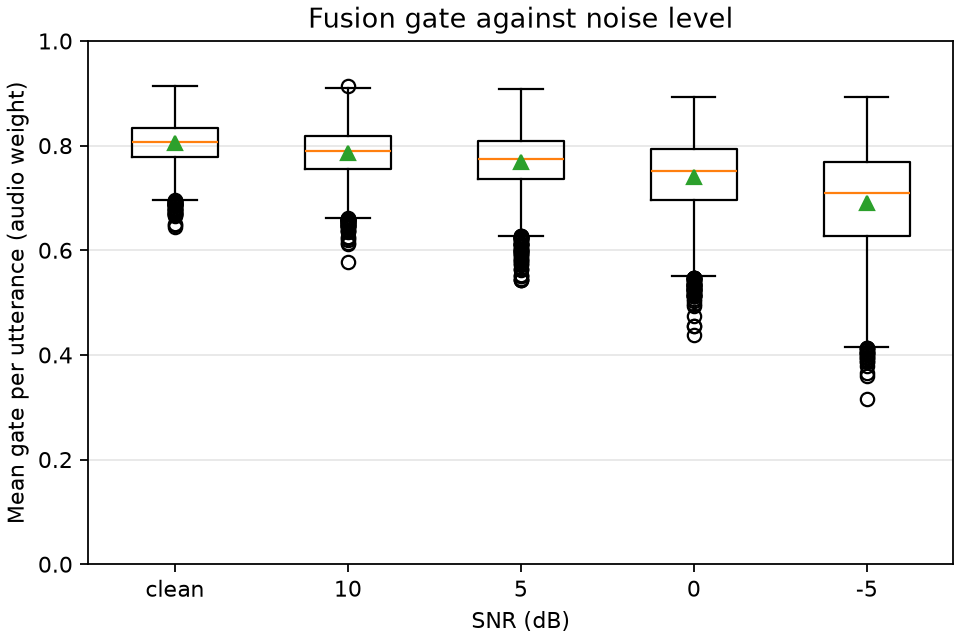
\includegraphics[width=0.8\textwidth]{reports/gate_analysis/gate_boxplot.png}
\caption{Per-utterance mean fusion gate $g_t$ at each SNR for P4. The gate falls monotonically from 0.804 (clean) to 0.691 ($-5$\,dB). Source: \texttt{reports/gate\_analysis/}.}
\label{fig:gate-boxplot}
\end{figure}

\begin{figure}[htbp]
\centering
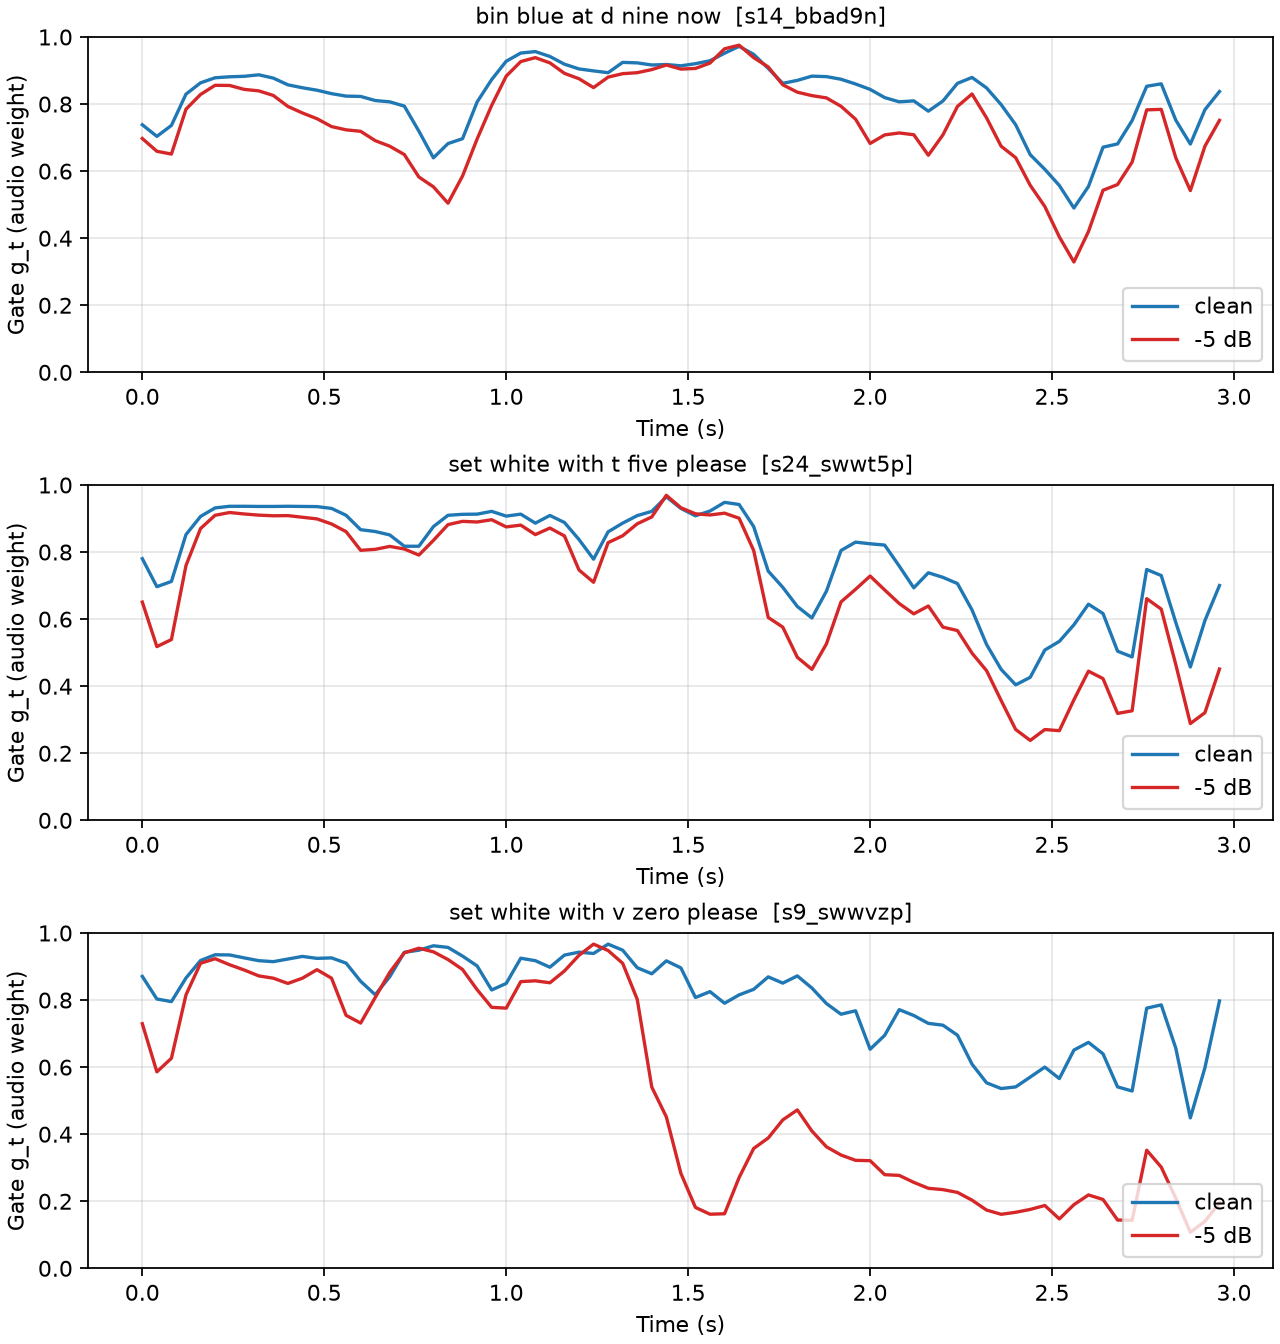
\includegraphics[width=0.8\textwidth]{reports/gate_analysis/gate_per_frame_examples.png}
\caption{Per-frame gate for example utterances at clean and $-5$\,dB. The gate drops during noisy stretches. Source: \texttt{reports/gate\_analysis/}.}
\label{fig:gate-per-frame}
\end{figure}

% ===== FINDINGS =====

\subsection{Key findings}

\begin{enumerate}
\item \textbf{Clean-condition target met:} P4 achieves 1.02\% WER on clean GRID audio, well below the 10\% target.
\item \textbf{Noise robustness:} P4 degrades gracefully from 1.02\% (clean) to 5.34\% ($-5$\,dB), outperforming B1 (1.96\% $\to$ 9.45\%) at every SNR.
\item \textbf{Lips are used when audio fails:} The fusion gate shifts from 0.80 (clean) to 0.69 ($-5$\,dB), and P4's video-only fallback (31.57\%) is far better than B3 v2's collapse (75.31\%).
\item \textbf{Modality dropout helps:} X1 (no dropout) is worse than P4 at all SNRs, especially $-5$\,dB (6.33\% vs 5.34\%).
\item \textbf{Attention + gating matters:} X2 (concat instead of attention) is close on clean audio but worse at $-5$\,dB (5.89\% vs 5.34\%).
\item \textbf{3D front-end matters most at low SNR:} X3 (2D instead of 3D) shows the largest degradation at $-5$\,dB (7.50\% vs 5.34\%).
\item \textbf{Consistent across speakers:} P4 beats B1 and B3 v2 on all four test speakers at every condition.
\item \textbf{Statistically significant:} Paired bootstrap confirms P4's advantage over B1 excludes 0 at 10, 5, 0 and $-5$\,dB.
\end{enumerate}
% Author: Cole Rodney Migisha (F-04, F-11).
\section{Real-World Speech}
\label{sec:realworld}
% TODO (F-04): twin_v5 vs ws_v5 on the film and TED test sets at clean, 0, -5, -10 dB, greedy
% and beam + LM; edge-word vs inner-word error; v6 (audio that does not belong to the face) as a
% negative result. Sources: reports/flix_v5/, reports/flix_v6/, reports/flix_v5/final_decoder.md.

% Author: Lisa Lusinga Namugenyi with Cole Rodney Migisha (F-11).
\section{Limitations and Future Work}
\label{sec:limitations}
% TODO (F-11): GRID's closed 51-word vocabulary and studio recordings; synthetic noise; edge
% words in real clips; voices that do not belong to the face (an audio-visual synchrony signal);
% frontal faces only; latency on CPU.

% Author: Charis Opol (F-11).
\section{Conclusion}
\label{sec:conclusion}
% TODO (F-11): answer the two research questions in one paragraph each.


\bibliographystyle{IEEEtran}
\bibliography{references}

\EOD
\end{document}
